\documentclass[a4paper, 12pt]{article}
\usepackage{geometry}
\geometry{verbose,a4paper,tmargin=2cm,bmargin=2cm,lmargin=2cm,rmargin=2cm}
\usepackage[T2A]{fontenc}
\usepackage[utf8]{inputenc}
\usepackage[english,russian]{babel}
\newif\ifisinsp
\newif\ifisone
\newif\ifisname
\isinsptrue
\isonetrue
\isnamefalse
\def \labtype {Лабораторная}
% Это для нумерации страниц после титульника
\usepackage{fancyhdr}
\pagestyle{fancy}
\renewcommand{\headrulewidth}{0pt}
\fancyfoot[C] {\thepage}

\usepackage{hyperref}
\hypersetup{pdftex,colorlinks=true,allcolors=black}
\usepackage{hypcap}

\usepackage{graphicx}
\usepackage{adjustbox}
\usepackage{multirow}

\def \labtype {Курсовая}
\def \labsubj {Системы баз данных}
\def \labauthor {Айтуганов Д. А. \\ Чебыкин И. Б.}
\def \labgroup {P3301}
\def \labinsp {Беликов П. А.}
\def \labname{Разработка базы данных сети магазинов}
\isonefalse
\isnametrue
\isnumfalse

% https://en.wikibooks.org/wiki/LaTeX/Source_Code_Listings
\usepackage{listings}
\usepackage{color}
\definecolor{mygreen}{rgb}{0,0.6,0}
\definecolor{mygray}{rgb}{0.5,0.5,0.5}
\definecolor{mymauve}{rgb}{0.58,0,0.82}
\definecolor{lightgray}{rgb}{.9,.9,.9}
\definecolor{darkgray}{rgb}{.4,.4,.4}
\definecolor{purple}{rgb}{0.65, 0.12, 0.82}

\lstdefinelanguage{JavaScript}{
  keywords={typeof, new, true, false, catch, function, return, null, catch, switch, var, if, in, while, do, else, case, break},
  keywordstyle=\ttfamily\color{blue}\bfseries,
  ndkeywords={class, export, boolean, throw, implements, import, this},
  ndkeywordstyle=\ttfamily\color{darkgray}\bfseries,
  identifierstyle=\ttfamily\color{black},
  sensitive=false,
  comment=[l]{//},
  morecomment=[s]{/*}{*/},
  commentstyle=\color{purple}\ttfamily,
  stringstyle=\color{red}\ttfamily,
  morestring=[b]',
  morestring=[b]"
}


\lstdefinelanguage{CSS}{
  morekeywords={accelerator,azimuth,background,background-attachment,
    background-color,background-image,background-position,
    background-position-x,background-position-y,background-repeat,
    behavior,border,border-bottom,border-bottom-color,
    border-bottom-style,border-bottom-width,border-collapse,
    border-color,border-left,border-left-color,border-left-style,
    border-left-width,border-right,border-right-color,
    border-right-style,border-right-width,border-spacing,
    border-style,border-top,border-top-color,border-top-style,
    border-top-width,border-width,bottom,caption-side,clear,
    clip,color,content,counter-increment,counter-reset,cue,
    cue-after,cue-before,cursor,direction,display,elevation,
    empty-cells,filter,float,font,font-family,font-size,
    font-size-adjust,font-stretch,font-style,font-variant,
    font-weight,height,ime-mode,include-source,
    layer-background-color,layer-background-image,layout-flow,
    layout-grid,layout-grid-char,layout-grid-char-spacing,
    layout-grid-line,layout-grid-mode,layout-grid-type,left,
    letter-spacing,line-break,line-height,list-style,
    list-style-image,list-style-position,list-style-type,margin,
    margin-bottom,margin-left,margin-right,margin-top,
    marker-offset,marks,max-height,max-width,min-height,
    min-width,-moz-binding,-moz-border-radius,
    -moz-border-radius-topleft,-moz-border-radius-topright,
    -moz-border-radius-bottomright,-moz-border-radius-bottomleft,
    -moz-border-top-colors,-moz-border-right-colors,
    -moz-border-bottom-colors,-moz-border-left-colors,-moz-opacity,
    -moz-outline,-moz-outline-color,-moz-outline-style,
    -moz-outline-width,-moz-user-focus,-moz-user-input,
    -moz-user-modify,-moz-user-select,orphans,outline,
    outline-color,outline-style,outline-width,overflow,
    overflow-X,overflow-Y,padding,padding-bottom,padding-left,
    padding-right,padding-top,page,page-break-after,
    page-break-before,page-break-inside,pause,pause-after,
    pause-before,pitch,pitch-range,play-during,position,quotes,
    -replace,richness,right,ruby-align,ruby-overhang,
    ruby-position,-set-link-source,size,speak,speak-header,
    speak-numeral,speak-punctuation,speech-rate,stress,
    scrollbar-arrow-color,scrollbar-base-color,
    scrollbar-dark-shadow-color,scrollbar-face-color,
    scrollbar-highlight-color,scrollbar-shadow-color,
    scrollbar-3d-light-color,scrollbar-track-color,table-layout,
    text-align,text-align-last,text-decoration,text-indent,
    text-justify,text-overflow,text-shadow,text-transform,
    text-autospace,text-kashida-space,text-underline-position,top,
    unicode-bidi,-use-link-source,vertical-align,visibility,
    voice-family,volume,white-space,widows,width,word-break,
    word-spacing,word-wrap,writing-mode,z-index,zoom},
  morestring=[s]{:}{;},
  sensitive,
  morecomment=[s]{/*}{*/}
}

% злостный костылище
% http://roman.khimov.ru/2011/05/19/latex-listings-cyrillic/
\lstset{
literate={а}{{\selectfont\char224}}1
{б}{{\selectfont\char225}}1
{в}{{\selectfont\char226}}1
{г}{{\selectfont\char227}}1
{д}{{\selectfont\char228}}1
{е}{{\selectfont\char229}}1
{ё}{{\"e}}1
{ж}{{\selectfont\char230}}1
{з}{{\selectfont\char231}}1
{и}{{\selectfont\char232}}1
{й}{{\selectfont\char233}}1
{к}{{\selectfont\char234}}1
{л}{{\selectfont\char235}}1
{м}{{\selectfont\char236}}1
{н}{{\selectfont\char237}}1
{о}{{\selectfont\char238}}1
{п}{{\selectfont\char239}}1
{р}{{\selectfont\char240}}1
{с}{{\selectfont\char241}}1
{т}{{\selectfont\char242}}1
{у}{{\selectfont\char243}}1
{ф}{{\selectfont\char244}}1
{х}{{\selectfont\char245}}1
{ц}{{\selectfont\char246}}1
{ч}{{\selectfont\char247}}1
{ш}{{\selectfont\char248}}1
{щ}{{\selectfont\char249}}1
{ъ}{{\selectfont\char250}}1
{ы}{{\selectfont\char251}}1
{ь}{{\selectfont\char252}}1
{э}{{\selectfont\char253}}1
{ю}{{\selectfont\char254}}1
{я}{{\selectfont\char255}}1
{А}{{\selectfont\char192}}1
{Б}{{\selectfont\char193}}1
{В}{{\selectfont\char194}}1
{Г}{{\selectfont\char195}}1
{Д}{{\selectfont\char196}}1
{Е}{{\selectfont\char197}}1
{Ё}{{\"E}}1
{Ж}{{\selectfont\char198}}1
{З}{{\selectfont\char199}}1
{И}{{\selectfont\char200}}1
{Й}{{\selectfont\char201}}1
{К}{{\selectfont\char202}}1
{Л}{{\selectfont\char203}}1
{М}{{\selectfont\char204}}1
{Н}{{\selectfont\char205}}1
{О}{{\selectfont\char206}}1
{П}{{\selectfont\char207}}1
{Р}{{\selectfont\char208}}1
{С}{{\selectfont\char209}}1
{Т}{{\selectfont\char210}}1
{У}{{\selectfont\char211}}1
{Ф}{{\selectfont\char212}}1
{Х}{{\selectfont\char213}}1
{Ц}{{\selectfont\char214}}1
{Ч}{{\selectfont\char215}}1
{Ш}{{\selectfont\char216}}1
{Щ}{{\selectfont\char217}}1
{Ъ}{{\selectfont\char218}}1
{Ы}{{\selectfont\char219}}1
{Ь}{{\selectfont\char220}}1
{Э}{{\selectfont\char221}}1
{Ю}{{\selectfont\char222}}1
{Я}{{\selectfont\char223}}1
}
\lstset{ %
	backgroundcolor=\color{white},   % choose the background color; you must add \usepackage{color} or \usepackage{xcolor}
	basicstyle=\ttfamily\footnotesize,        % the size of the fonts that are used for the code
	breakatwhitespace=false,         % sets if automatic breaks should only happen at whitespace
	breaklines=true,                 % sets automatic line breaking
	captionpos=b,                    % sets the caption-position to bottom
	commentstyle=\color{black},    % comment style
	deletekeywords={...},            % if you want to delete keywords from the given language
	escapeinside={\%*}{*)},          % if you want to add LaTeX within your code
	extendedchars=true,              % lets you use non-ASCII characters; for 8-bits encodings only, does not work with UTF-8
	keepspaces=true,                 % keeps spaces in text, useful for keeping indentation of code (possibly needs columns=flexible)
	keywordstyle=\color{blue},       % keyword style
	language=Octave,                 % the language of the code
	otherkeywords={*,...},            % if you want to add more keywords to the set
	rulecolor=\color{black},         % if not set, the frame-color may be changed on line-breaks within not-black text (e.g. comments (green here))
	showspaces=false,                % show spaces everywhere adding particular underscores; it overrides 'showstringspaces'
	showstringspaces=false,          % underline spaces within strings only
	showtabs=false,                  % show tabs within strings adding particular underscores
	stepnumber=2,                    % the step between two line-numbers. If it's 1, each line will be numbered
	stringstyle=\color{mymauve},     % string literal style
	tabsize=2,	                   % sets default tabsize to 2 spaces
}

\lstset{
	caption=,
	basicstyle=\ttfamily\selectfont\scriptsize
}
\begin{document}
\begin{titlepage}
	\begin{center}
		\large
		Университет ИТМО

		\vspace{0.25cm}
		
		Факультет программной инженерии и компьютерной техники
		
		Кафедра вычислительной техники
		\vfill
		
		\textsc{\labtype\spaceработа \ifisnum № \labnum{} \fi по дисциплине \\"\labsubj" \ifisname\small \\ \labname \fi}
			
		\bigskip
	\end{center}
	\vfill
	\vfill
	
	\begin{flushright}
	\ifisone
	Выполнил: \labauthor
	\else
	Выполнили: \labauthor
	\fi

	\vspace{0.25cm}
	Группа: \labgroup
			
	\vspace{0.25cm}
	\ifisinsp
	Проверяющий: \labinsp
	\fi
	\end{flushright}
	\vfill
	
	\begin{center}
	СПб, \the\year
	\end{center}
\end{titlepage}

\tableofcontents
\newpage
\section{Описание предметной области}
В качестве предметной области была выбрана сеть магазинов, которые продают
различные товары. В модели учитываются расписание сотрудников, логирование
продаж, категории товаров и т. д.
\section{Модель первой части}
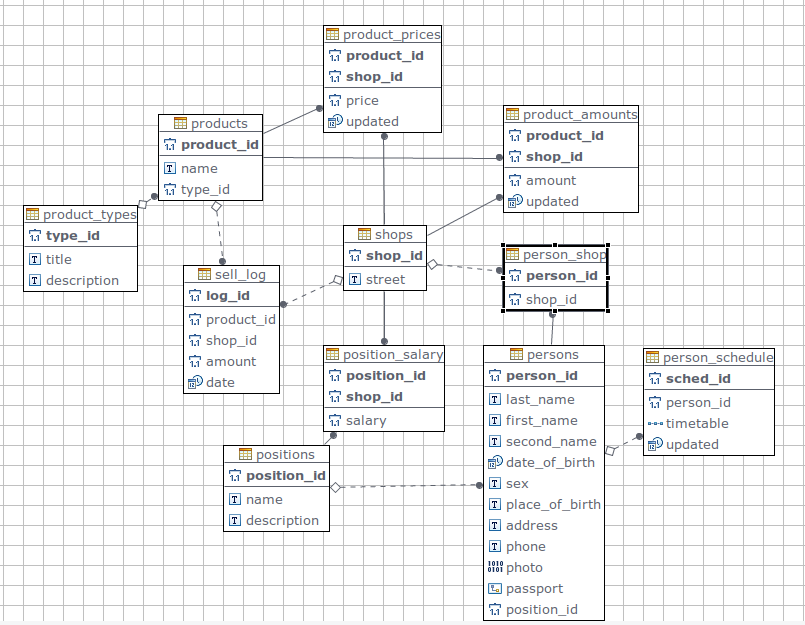
\includegraphics[width=\textwidth]{img/diagram.png}
\subsection{Примеры CRUD-кода}
\subsubsection{Хранимые процедуры}
\begin{verbatim}
CREATE FUNCTION add_product(name text, type_id integer) RETURNS integer
    LANGUAGE sql
    AS $$
INSERT INTO products VALUES(NULL, name, type_id) RETURNING product_id;
 $$;
\end{verbatim}

\subsubsection{API на прикладном языке программирования}
\begin{lstlisting}[language=Java]
    private <R extends UpdatableRecord, T extends TableImpl<R>, F extends TableField<R, Integer>>
    int doCommand(T table, F[] pkey, CmdType type, int[] id, String fieldName, Object[] args, boolean skip_id) {
        R record = null;
        if (type == CmdType.ADD || type == CmdType.FIELDS) {
            record = ctx.newRecord(table);
        }

        if (type == CmdType.READ || type == CmdType.UPDATE || type == CmdType.DELETE) {
            if (pkey.length == 1) {
                record = ctx.fetchOne(table, pkey[0].equal(id[0]));
            } else {
                record = ctx.fetchOne(table, pkey[0].equal(id[0]).and(pkey[1].equal(id[1])));
            }
            if (record == null && type != CmdType.READ) {
                throw new IllegalArgumentException("No such row");
            }
        }
        if (type == CmdType.DELETE) {
            record.delete();
            return 0;
        }

        if (type == CmdType.READ) {
            if( id[0] > 0 && record == null ){
                throw new IllegalArgumentException("No such row");
            }
            Result<R> records;
            if( record != null ) {
                records = ctx.newResult(table);
                records.add(record);
            }else{
                records = ctx.fetch(table);
            }
            boolean printed = false;
            for (R r : records) {
                if (fieldName != null) {
                    Object data = r.getValue(fieldName);
                    System.out.println(data);
                } else {
                    if( !printed ) {
                        for (Field<?> f : r.fields()) {
                            System.out.print(f.getName()+" ");
                        }
                        printed = true;
                        System.out.println();
                    }
                    for (Field<?> f : r.fields()) {
                        Object data = r.getValue(f);
                        System.out.print(data + " ");
                    }
                    System.out.println();
                }
            }
            return 0;
        }

        Field<?>[] fields = record.fields();
        if (type == CmdType.FIELDS) {
            for (Field f : fields) {
                System.out.println(f);
            }
            return 0;
        }
        int i = skip_id ? -id.length : 0;
        for (Field f : fields) {
            // Skip id
            if (i < 0) {
                i++;
                continue;
            }
            record.set(f, args[i++]);
            System.out.println(f);
        }
        record.store();
        return (int) record.getValue(0);
    }
\end{lstlisting}

\section{Схема второй части}
\begin{lstlisting}[language=Javascript]
persons
var mongoose = require('mongoose');
var table = 'persons';
var schema = mongoose.Schema({
	last_name: {type: String, required: true},
	first_name: {type: String, required: true},
	second_name: String,
	date_of_birth: {type: String, required: true},
	sex: {type: String, validate: /M|F/},
	place_of_birth: {type: String, required: true},
	address: {type: String, required: true},
	phone: {type: String, required: true},
	photo: Buffer,
	passport: {
		type: String,
		unique: true,
		validate: /\d{4},\d{6}/,
		required: true
	},
	position: {
		name: {type: String, required: true},
		description: String,
		shop_id: {
			type: Number,
			required: true
		},
		salary: {type: Number, required: true},
	}
});

module.exports = {
	schema: schema,
	model: mongoose.model(table, schema)
}

products
var mongoose = require('mongoose');
var table = 'products';
var schema = mongoose.Schema({
	name: {type: String, index: {unique: true}},
	type: {
		name: {type: String, required: true},
		description: String
	},
	sell_info: {
		shop_id: Number,
		price: Number,
		amount: Number,
	}
});

module.exports = {
	schema: schema,
	model: mongoose.model(table, schema)
}

sell_logs
var mongoose = require('mongoose');
var table = 'sell_log';
var schema = mongoose.Schema({
	name: {type: String, index: {unique: true} },
	product_id: { type: Number, unique: true },
	shop_id: { type: Number, unique: true },
	amount: Number,
	date: Date,
});

module.exports = {
	schema: schema,
	model: mongoose.model(table, schema)
}

shops
var mongoose = require('mongoose');
var table = 'shops';
var schema = mongoose.Schema({
	street: {
		type: String,
		required: true
	},
	number: {
		type: Number,
		required: true,
	},
});
schema.index({street: 1, number: 1}, {unique: true});
module.exports = {
	schema: schema,
	model: mongoose.model(table, schema)
}
\end{lstlisting}

\subsection{Примеры CRUD-кода}
\begin{lstlisting}[language=Javascript]
'add': function(splitted_input) {
	var schema = get_schema_by_name(splitted_input[1]);
	if(schema == null) return;
	model = fill_fields(schema, null);
	console.log(model);
	model.save((err) => print_errors(err));
}
\end{lstlisting}

\section{Модели взамодействия с Redis}
\subsection{Первая часть}
При выполнении read операции результат запроса сохраняется для конкретной команды.
При выполнении add, update или delete, кэш очищается.
\subsection{Вторая часть}
При выполнении read операции запрос кэшируется на определенный промежуток времени.

\end{document}
